%%%%%%%%%%%%%%%%%%%%%%%%%%%%%%%%%%%%%%%%%
\section{Agenda}
\begin{frame}{Agenda}
\begin{itemize}
\item Problem introduktion
\item Eksisterende modeller
\item Parameter bestemmelse
\item Test \& målinger
\item Data behandling
\item Ny model
\item Konklusion
\end{itemize}
\end{frame}
%%%%%%%%%%%%%%%%%%%%%%%%%%%%%%%%%%%%%%%%%
\section{Problem introduktion}
\begin{frame}{Problem introduktion}
\begin{minipage}{0.5\textwidth}

\begin{itemize}
\item Lavstående antenner.
\item Jorden og andre objekters påvirkning kan ikke længere negleres.
\end{itemize}

\end{minipage}
\begin{minipage}{0.45\textwidth}

%Find fedt billede

\end{minipage}
\end{frame}

%%%% Signaler
\begin{frame}{Problem introduktion}
\begin{minipage}{0.5\textwidth}

\begin{itemize}
\item Direct wave
\item Reflected wave
\item Surface wave
\end{itemize}

\end{minipage}
\begin{minipage}{0.45\textwidth}

%Find fedt billede

\end{minipage}
\end{frame}

%%%% Andre effekter
\begin{frame}{Problem introduktion}
\begin{minipage}{0.5\textwidth}

\begin{itemize}
\item Line of sight (LOS)
\item Far field og Near field
\item Scattering
\end{itemize}

\end{minipage}
\begin{minipage}{0.45\textwidth}

%Find fedt billede

\end{minipage}
\end{frame} 
 
 
%%%%%%%%%%%%%%%%%%%%%%%%%%%%%%%%%%%%%%%
\section{Exiterende modeller}
\begin{frame}{Exiterende modeller}
\begin{minipage}{.45\textwidth}
\raggedright\textcolor{thomasblue}{\textbf{Friss free space PL (FSPL)}:}
\begin{itemize}
\item Only direct wave
\item High heights
\end{itemize} 

\vspace{1em}
\textcolor{black}{\textbf{Conditions:}}
\begin{itemize}
\item No Multipath
\item $d >> \lambda$
\end{itemize}
\end{minipage}
\begin{minipage}{0.5\textwidth}

\begin{figure}[!htbp]
 \centering
  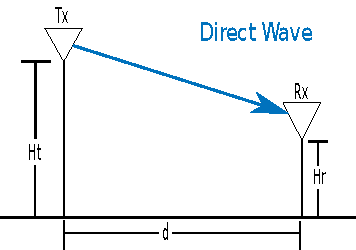
\includegraphics[width = \columnwidth]{figures/friss_illu.pdf}
  \end{figure}
\end{minipage}

\vspace{1em}
\begin{equation*}
L_p=\left(\frac{4 \pi d}{\lambda}\right)^2
\end{equation*}
\end{frame}


\begin{frame}{Exiterende modeller}
\begin{minipage}{.45\textwidth}
\raggedright\textcolor{thomasred}{\textbf{Approximated two-ray}}\\
\raggedright\textcolor{thomasred}{\textbf{ground-reflection PL (ATRPL)}:}
\begin{itemize}
\item Direct and reflected wave
\item Medium heights
\end{itemize} 

\vspace{1em}
\textcolor{black}{\textbf{Conditions:}}
\begin{itemize}
\item No obstacles
\item Plane surface
\item $d > \frac{4\pi \cdot h_t h_r }{\lambda}$
\end{itemize}

\end{minipage}
\begin{minipage}{0.5\textwidth}
\begin{figure}[!htbp]
 \centering
  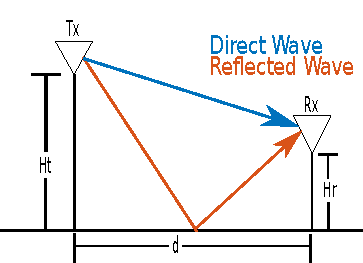
\includegraphics[width = \columnwidth]{figures/two_ray_illu.pdf}
  \end{figure}
\end{minipage}

\vspace{1em}
\begin{equation*}
L_{p} = \left(\frac{d^2}{h_t h_r}\right)^2
\label{two_ray_model}
\end{equation*}
\end{frame}


\begin{frame}{Exiterende modeller}
\begin{minipage}{.45\textwidth}
\raggedright\textcolor{thomasgreen}{\textbf{Norton surface wave PL (NSPL)}:}
\begin{itemize}
\item Only surface wave
\item Low heights
\item Dependent on surface constants
\end{itemize}

\vspace{1em}
\textcolor{black}{\textbf{Conditions:}}
\begin{itemize}
\item No obstacles
\item Plane surface
\item $h_t,h_r > \lambda$
\end{itemize}

\end{minipage}%
\begin{minipage}{0.5\textwidth}
\begin{figure}[!htbp]
 \centering
  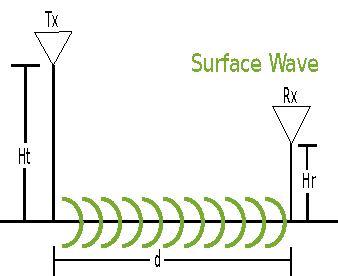
\includegraphics[width = \columnwidth]{figures/surf_illu.pdf}
  \end{figure}
\end{minipage}

\vspace{1em}
\begin{equation}
L_p=\left({d} \cdot \left|\frac{\lambda}{2\pi z}\right|^{-1}\right)^4
\label{surface_wave}
\end{equation}
\end{frame}



\begin{frame}{Exiterende modeller}
\begin{minipage}{.45\textwidth}
\raggedright\textcolor{thomaspurple}{\textbf{Ground wave PL (GWPL)}:}
\begin{itemize}
\item All waves
\item All heights
\item Dependent on surface constants
\end{itemize} 

\vspace{1em}
\textcolor{black}{\textbf{Conditions:}}
\begin{itemize}
\item No obstacles
\item Plane surface
\end{itemize}

\end{minipage}
\begin{minipage}{0.5\textwidth}
\begin{figure}[!htbp]
 \centering
  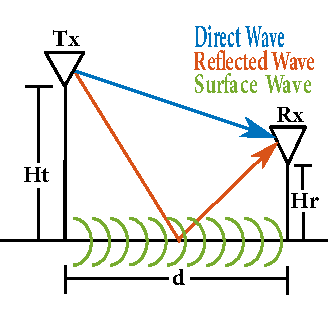
\includegraphics[width = \columnwidth]{figures/poster_cropped_1.pdf}
  \end{figure}
\end{minipage}

\vspace{1em}
\begin{equation}
L_p=\left(\frac{4 \pi d}{\lambda}\right)^2 \cdot \Big|\underbrace{1}_{\begin{subarray}{c}Direct\\wave\end{subarray}}+\underbrace{R\text{e}^{j\Delta}}_{\begin{subarray}{c}Reflected\\wave\end{subarray}}+\underbrace{(1-R)A\text{e}^{j\Delta}}_{\begin{subarray}{c}Surface\\wave\end{subarray}}\Big|^{-2} 
\label{ground_wave}
\end{equation}
\end{frame}

%%%%%%%%%%%%%%%%%%%%%%%%%%%%%%%%%%%%
\section{Parameter bestemmelse}
\begin{frame}{Measurements}
\begin{figure}[!htbp]
	\centering
	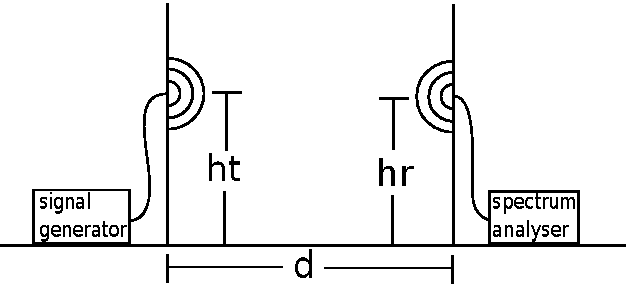
\includegraphics[width = 0.8\columnwidth]{figures/setup.pdf}
\end{figure}
\begin{minipage}{0.15\textwidth}
 \textcolor{white}{.}  
\end{minipage}%
\begin{minipage}{0.8\textwidth}
\begin{itemize}
\item Frequency
\item Antenna sets
\item Polarization
\item Location
\item Rx/Tx heights
\item Distances
\end{itemize}
\end{minipage}
\end{frame}



\section{Parameter bestemmelse}
\begin{frame}{Measurements}
\begin{figure}[!htbp]
	\centering
	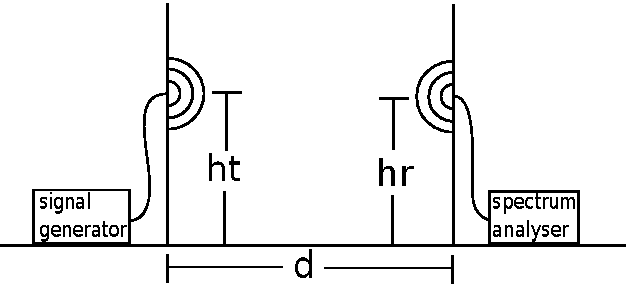
\includegraphics[width = 0.8\columnwidth]{figures/setup.pdf}
\end{figure}
\begin{minipage}{0.15\textwidth}
 \textcolor{white}{.}  
\end{minipage}%
\begin{minipage}{0.8\textwidth}
\begin{itemize}
\item 1 Frequency (858 MHz)
\item 2 Antenna sets (monopole and patch)
\item 2 Polarization (horizontal and vertical)
\item 2 Location (outdoor and indoor)
\item 4 Rx/Tx heights (from 0.04 to 2.02 m)
\item 6 Distances (from 1 to 30 m)
\item Total count : 4800 measurements
\end{itemize}
\end{minipage}
\end{frame}